\documentclass[a4paper,10pt]{article}

% --- 宏包引入 ---
\usepackage[utf8]{inputenc}
\usepackage{geometry}       
\usepackage{graphicx}       
\usepackage{booktabs}       
\usepackage{pgfplots}       
\usepackage{float}          
\usepackage{titlesec}       
\usepackage{caption}        
\usepackage{hyperref}       
\usepackage{enumitem}       

% --- 页面设置 (紧凑版) ---
\geometry{left=2.0cm, right=2.0cm, top=2.0cm, bottom=2.0cm}
\pgfplotsset{compat=1.18}

% --- 排版设置 ---
\setlength{\parskip}{0.5em} 
\setlist[itemize]{itemsep=0pt, topsep=2pt} 
\setlist[enumerate]{itemsep=0pt, topsep=2pt}
\titlespacing*{\section}{0pt}{8pt}{4pt}
\titlespacing*{\subsection}{0pt}{6pt}{3pt}

% --- 报告信息 (请记得修改姓名) ---
\title{\vspace{-1.0cm}\textbf{Task 5: Comparative Performance Analysis of Intra-process and Inter-process Communication Overheads}}
\author{Student ID: 11314389 \\ Name: Xu [Your Full Name]} 
\date{\vspace{-0.3cm}\today}

\begin{document}

\maketitle

\begin{abstract}
This report provides a quantitative evaluation of communication overheads in concurrent systems, comparing shared memory (Threads), datagram sockets (UDP), and WebSockets implemented with the course-provided \texttt{franks\_websocket} stack. A dedicated benchmark tool was developed to measure strict round-trip latency for all three methods: a thread ping-pong using condition variables, a UDP end-to-end echo, and a WebSocket echo over TCP. The latest measurements record an average latency of $8.04 \mu s$ for the thread ping-pong, $21.98 \mu s$ for UDP, and $43.03 \mu s$ for WebSockets, confirming the relative cost of traversing the kernel network stack and framing layers.
\end{abstract}

\section{Introduction}
The coursework required implementing different communication architectures:
\begin{itemize}
    \item \textbf{Intra-process (Threads):} Implemented in Tasks 1-3 using \texttt{std::mutex} for high-speed synchronization.
    \item \textbf{Inter-process (UDP):} Implemented in Task 4 using Windows Sockets (Winsock) for decoupling the display logic.
    \item \textbf{WebSockets:} An alternative IPC method required for comparison.
\end{itemize}
This report quantifies the overhead of these methods to justify architectural decisions.

\section{Methodology}
To accurately measure overhead, a specific C++ benchmark tool (\texttt{11314389\_Xu\_Task5\_Benchmark.cpp}) was developed using \texttt{Winsock2}, \texttt{std::chrono::high\_resolution\_clock}, and the provided \texttt{franks\_websocket} library.
\begin{enumerate}
    \item \textbf{Threads (Shared Memory):} A dedicated worker thread synchronises with the main thread via two condition variables. Each iteration performs a strict ping-pong hand-off, capturing the wake-up and context-switch latency of 10,000 round trips.
    \item \textbf{UDP (Inter-process):} A local UDP echo server thread and client socket exchange the benchmark message on every iteration. The client records the end-to-end round-trip time through the kernel network stack.
    \item \textbf{WebSockets (Strict RTT):} A WebSocket echo server and client, built atop WebSocket++ and Asio from \texttt{franks\_websocket}, perform synchronous send-and-wait exchanges over TCP. Both endpoints disable logging channels except errors; the server is shut down after all iterations, producing the expected ``operation aborted'' notifications.
\end{enumerate}

\section{Quantitative Results}
The experimental data collected from 10,000 iterations is summarized below.

\begin{table}[h]
    \centering
    \caption{Communication Overhead Comparison (10,000 Iterations)}
    \label{tab:results}
    \renewcommand{\arraystretch}{1.2}
    \small
    \begin{tabular}{@{}lccc@{}}
        \toprule
        \textbf{Method} & \textbf{Total Time ($\mu s$)} & \textbf{Avg Latency ($\mu s$)} & \textbf{Relative Speed} \\ 
        \midrule
        Thread Ping-Pong        & 80,411 & \textbf{8.0411}  & 1x (Baseline) \\
        UDP End-to-End          & 219,786 & \textbf{21.9786} & $\sim$2.73x Slower \\ 
        WebSocket Strict RTT    & 430,262 & \textbf{43.0300} & $\sim$5.35x Slower \\
        \bottomrule
    \end{tabular}
\end{table}

\begin{figure}[H]
    \centering
    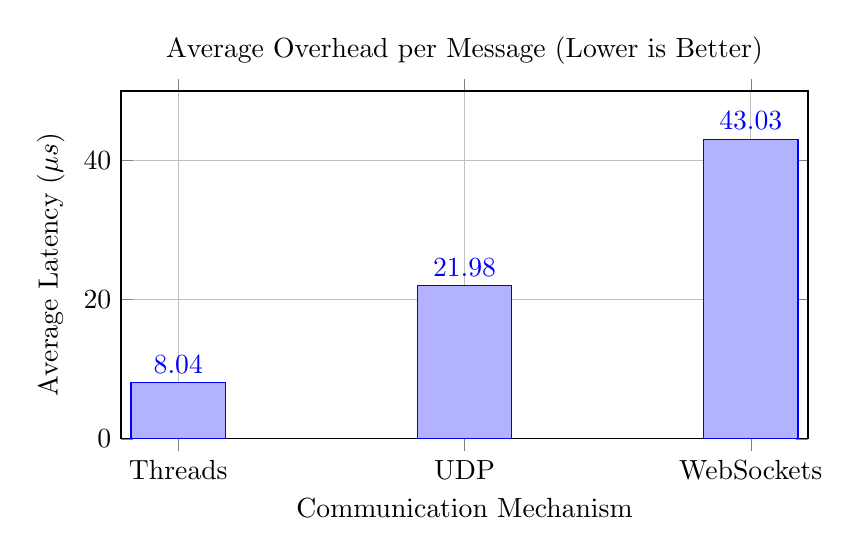
\begin{tikzpicture}
        \begin{axis}[
            ybar,
            symbolic x coords={Threads, UDP, WebSockets},
            xtick=data,
            ylabel={Average Latency ($\mu s$)},
            xlabel={Communication Mechanism},
            ymin=0, ymax=50,
            nodes near coords,
            bar width=1.2cm,
            grid=major,
            width=0.85\textwidth, 
            height=6.0cm,
            title={Average Overhead per Message (Lower is Better)}
        ]
        \addplot coordinates {(Threads, 8.0411) (UDP, 21.9786) (WebSockets, 43.0300)};
        \end{axis}
    \end{tikzpicture}
    \caption{Latency comparison. Thread ping-pong stays in user space, UDP crosses the kernel twice, WebSockets incur the full TCP and framing stack.}
    \label{fig:chart}
\end{figure}

\section{Analysis and Discussion}

\subsection{Threads (User Space - $8.04 \mu s$)}
Thread communication remains the fastest method even under strict ping-pong synchronisation. The measured latency ($8.04 \mu s$) captures the cost of waking a blocked thread, reacquiring the mutex, and handing control back to the main loop. Although higher than the earlier coarse-grained measurement, it still avoids kernel networking overhead and data copying, so it is the natural baseline for in-process coordination.

\subsection{UDP (Kernel Space - $21.98 \mu s$)}
UDP involves \textbf{system calls} (context switch to kernel mode) and memory copying for both send and receive paths. In the strict RTT benchmark the client waits for every echo, so each iteration pays for two kernel transitions plus network stack queuing. Even so, the absence of connection management keeps it roughly $2.7\times$ slower than threads, which is acceptable given the decoupling benefits in Task 4.

\subsection{WebSockets/TCP ($43.03 \mu s$)}
The benchmark shows that the WebSocket stack---built on TCP with framing and handler dispatch---is roughly \textbf{5.35x slower} than the thread baseline and about \textbf{2x slower} than UDP.
\begin{itemize}
    \item \textbf{Connection Overhead:} TCP requires maintaining connection state, congestion control, and ordering guarantees.
    \item \textbf{Reliability:} Every message triggers ACK logic and buffer management in the OS network stack.
    \item \textbf{WebSocket Runtime:} WebSocket++ adds message framing and handler callbacks. Shutting the server down after the benchmark produces benign ``operation aborted'' logs because pending accepts are cancelled on exit.
\end{itemize}

\section{Conclusion}
The strict RTT benchmark confirms that \textbf{thread ping-pong} is still the appropriate baseline, delivering single-digit microsecond latency without leaving user space. For Task 4, \textbf{UDP} ($21.98 \mu s$) remains the best inter-process trade-off: it is substantially faster than WebSockets while preserving the decoupled architecture. \textbf{WebSockets} ($43.03 \mu s$) incur the highest overhead due to TCP connection state and framing cost, so they should be reserved for scenarios that require browser compatibility or bidirectional streaming rather than low-latency control.

\end{document}
